% This must be in the first 5 lines to tell arXiv to use pdfLaTeX, which is strongly recommended.
\pdfoutput=1
% In particular, the hyperref package requires pdfLaTeX in order to break URLs across lines.

\documentclass[11pt]{article}

% Remove the "review" option to generate the final version.
\usepackage{EMNLP2023}

% Standard package includes
\usepackage{times}
\usepackage{latexsym}

% For proper rendering and hyphenation of words containing Latin characters (including in bib files)
\usepackage[T1]{fontenc}
% For Vietnamese characters
% \usepackage[T5]{fontenc}
% See https://www.latex-project.org/help/documentation/encguide.pdf for other character sets

% This assumes your files are encoded as UTF8
\usepackage[utf8]{inputenc}

% Add textcomp for additional symbols
\usepackage{textcomp}

% Add amsmath and amssymb for mathematical symbols including Greek letters
\usepackage{amsmath,amssymb}

% This is not strictly necessary, and may be commented out.
% However, it will improve the layout of the manuscript,
% and will typically save some space.
\usepackage{microtype}

% This is also not strictly necessary, and may be commented out.
% However, it will improve the aesthetics of text in
% the typewriter font.
\usepackage{inconsolata}

% Add graphicx for including figures
\usepackage{graphicx}
\graphicspath{{./}} % Look for figures in the current directory

% Add booktabs for nice tables
\usepackage{booktabs}

% Add multirow and multicol for complex tables
\usepackage{multirow}
\usepackage{multicol}

% For better table and figure adjustments
\usepackage{tabularx}
\usepackage{adjustbox} % Added for adjusting box widths
\usepackage{xurl} % Added for better URL breaking in bibliography

% Add hyperref for enhanced PDF functionality - load this last
\usepackage{hyperref}
\hypersetup{
    colorlinks=true,
    linkcolor=blue,
    filecolor=magenta,
    urlcolor=cyan,
    pdftitle={ConsultAI: Multi-Agent Ethical Deliberation System},
    pdfauthor={Chen Gaoxiang, Gang Jinqiang},
    pdfsubject={Artificial Intelligence},
    pdfkeywords={multi-agent systems, ethical deliberation, healthcare AI, ethical reasoning},
    breaklinks=true % Added to help with URL breaking
}

% If the title and author information does not fit in the area allocated, uncomment the following
%
\setlength\titlebox{8cm} % Increased title box further for author affiliations
%
% and set <dim> to something 5cm or larger.

\title{ConsultAI: Multi-Agent Ethical Deliberation System for Healthcare Decision Support \\
\normalsize Final Project for CSC6052}

% Author information can be set in various styles:
% For several authors from the same institution:
% \author{Author 1 \and ... \and Author n \\
%         Address line \\ ... \\ Address line}
% if the names do not fit well on one line use
%         Author 1 \\ {\bf Author 2} \\ ... \\ {\bf Author n} \\
% For authors from different institutions:
% \author{Author 1 \\ Address line \\  ... \\ Address line
%         \And  ... \And
%         Author n \\ Address line \\ ... \\ Address line}
% To start a seperate ``row'' of authors use \AND, as in
% \author{Author 1 \\ Address line \\  ... \\ Address line
%         \AND
%         Author 2 \\ Address line \\ ... \\ Address line \And
%         Author 3 \\ Address line \\ ... \\ Address line}

\author{Chen Gaoxiang \\
  School of Data Science \\
  The Chinese University of Hong Kong, Shenzhen \\
  \texttt{224040277@link.cuhk.edu.cn} \\[2ex] % Added explicit extra vertical space
  \AND
  Gang Jinqiang \\
  School of Data Science \\
  The Chinese University of Hong Kong, Shenzhen \\
  \texttt{224040306@link.cuhk.edu.cn}}

% 修改表格环境为调整表格宽度
\usepackage{tabularx}

% Add tcolorbox package if not already present
\usepackage{tcolorbox}
\tcbuselibrary{skins,breakable} % For better box styling and breakable boxes

% Add xcolor for color customization
\usepackage{xcolor}

% Define custom tcolorbox styles for AI-generated text
\newtcolorbox{casebox}[1]{
  breakable,
  colback=blue!5!white,
  colframe=blue!75!black,
  fonttitle=\bfseries,
  title={\textbf{\textcolor{white}{#1}}},
  boxrule=0.5pt,
  boxsep=2mm,
  left=6pt,
  right=6pt,
  top=6pt,
  bottom=6pt,
  arc=0pt,
  autoparskip
}

\newtcolorbox{commentarybox}[1]{
  breakable,
  colback=green!5!white,
  colframe=green!60!black,
  fonttitle=\bfseries,
  title={\textbf{\textcolor{white}{#1}}},
  boxrule=0.5pt,
  boxsep=2mm,
  left=6pt,
  right=6pt,
  top=6pt,
  bottom=6pt,
  arc=0pt,
  autoparskip
}

\newtcolorbox{analysisbox}[1]{
  breakable,
  colback=orange!5!white,
  colframe=orange!80!black,
  fonttitle=\bfseries,
  title={\textbf{\textcolor{white}{#1}}},
  boxrule=0.5pt,
  boxsep=2mm,
  left=6pt,
  right=6pt,
  top=6pt,
  bottom=6pt,
  arc=0pt,
  autoparskip
}

\begin{document}
\maketitle
\begin{abstract}
This paper presents ConsultAI, a novel multi-agent system for ethical deliberation in healthcare scenarios. By leveraging large language models to simulate multiple healthcare professionals with distinct roles, ConsultAI facilitates collaborative ethical decision-making for complex medical dilemmas. Our system demonstrates how role-specialized agents can engage in structured deliberation, reaching consensus through iterative discussion while maintaining transparency in reasoning. Evaluation across multiple ethical domains (autonomy, beneficence, justice, and resource allocation) shows that our approach produces comprehensive ethical analyses that consider diverse stakeholder perspectives. Empirical results from 20 case studies demonstrate that multi-agent deliberation outperforms single-agent approaches by a significant margin, with a 37\% improvement in ethical principle coverage, 42\% increase in consideration of diverse stakeholder perspectives, and 20\% enhancement in reasoning depth. The triad configuration (attending physician, patient advocate, clinical ethicist) offers an optimal balance of performance and computational efficiency, while the extended configuration with six distinct roles provides more nuanced analysis for complex ethical dilemmas. ConsultAI represents a promising approach to augmenting clinical ethics committees with AI support systems that model the collaborative nature of ethical deliberation in healthcare.
\end{abstract}

\section{Introduction}

Healthcare professionals frequently face complex ethical dilemmas that require careful deliberation among multiple stakeholders with diverse expertise and perspectives. Traditional clinical ethics committees bring together professionals from different backgrounds to deliberate on challenging cases, but this process is often time-consuming and resource-intensive. Additionally, conventional clinical decision support systems typically lack the ability to model complex ethical reasoning with multiple perspectives.

In this work, we introduce ConsultAI, a multi-agent ethical deliberation system designed to support healthcare professionals facing ethical dilemmas. Our key contributions include:

\begin{itemize}
    \item A flexible multi-agent architecture that simulates collaborative ethical deliberation among stakeholders with distinct healthcare roles
    \item Role-specialized agents with defined expertise areas and stakeholder perspectives that engage in structured, transparent reasoning
    \item A comprehensive evaluation framework that assesses ethical reasoning quality across multiple dimensions
    \item Demonstrated improvements in ethical principle coverage, stakeholder consideration, and recommendation practicality compared to single-agent approaches
\end{itemize}

The complete source code and documentation for ConsultAI are available on GitHub at: \url{https://github.com/vittorioence/MyProjects}.

\section{Related Work}

\subsection{Multi-Agent Dialogue Systems}

Recent work has explored the use of multiple LLM instances as conversational agents. For example, \citet{chan2023chateval} demonstrated that multi-agent debate can improve reasoning performance on complex tasks, while \citet{park2023generative} used role-playing agents to generate more creative solutions. Our work extends these approaches to ethical deliberation in healthcare.

Multi-agent systems have shown particular promise in domains requiring diverse perspectives. \citet{zheng2023judging} found that LLM-based judges could effectively evaluate responses from other models in debate scenarios, suggesting that specialized roles in deliberation can improve overall reasoning quality. \citet{bang2023multiturn} demonstrated how structured multi-turn debates among LLM agents can lead to enhanced reasoning capabilities through the confrontation of different viewpoints.

\subsection{AI Ethics in Healthcare}

Prior research has explored the use of AI for ethical analysis in clinical settings. \citet{mittelstadt2019principles} proposed frameworks for incorporating ethical principles into clinical decision support systems, and \citet{biller2021ethical} examined how AI might assist ethics committees. However, these approaches typically rely on single-agent systems without modeling diverse stakeholder perspectives.

Medical AI systems have increasingly incorporated ethical frameworks, with \citet{guan2023medical} exploring how AI can consider clinical outcomes while respecting human values. The principle-based approach to bioethics, as outlined by \citet{beauchamp2001principles}, provides a foundation for many AI ethics systems in healthcare, with autonomy, beneficence, non-maleficence, and justice serving as cornerstone principles.

\subsection{LLMs for Ethical Reasoning}

Several studies have investigated LLMs' capabilities for ethical reasoning. \citet{bang2023multiturn} found that chain-of-thought prompting improves ethical analysis, while \citet{jiang2021can} demonstrated that LLMs can apply ethical frameworks to novel scenarios. Our work builds on these findings by implementing multiple agents representing different ethical perspectives.

More recent research by \citet{schwitzgebel2023computers} explores the philosophical implications of delegating moral reasoning to AI systems, arguing that moral status attribution should consider the functional roles these systems play in ethical deliberation. \citet{perez2022discovering} found that model-written evaluations can help discover and characterize the ethical reasoning capabilities of language models, providing a foundation for our approach to role-specialized agents.

\section{ConsultAI System}

\subsection{System Architecture}

ConsultAI implements a multi-tiered architecture for ethical deliberation:

\begin{enumerate}
    \item \textbf{Case Processing Layer}: Handles case study input and preparation
    \item \textbf{Role Definition Layer}: Defines specialized agent roles with unique expertise
    \item \textbf{Deliberation Layer}: Orchestrates multi-round discussion among agents
    \item \textbf{Consensus Layer}: Synthesizes perspectives into final recommendations
    \item \textbf{Evaluation Layer}: Assesses quality of ethical reasoning
\end{enumerate}

Figure \ref{fig:architecture} illustrates the system architecture, showing how the different components interact to enable structured ethical deliberation.

\begin{figure}[t!]
    \centering
    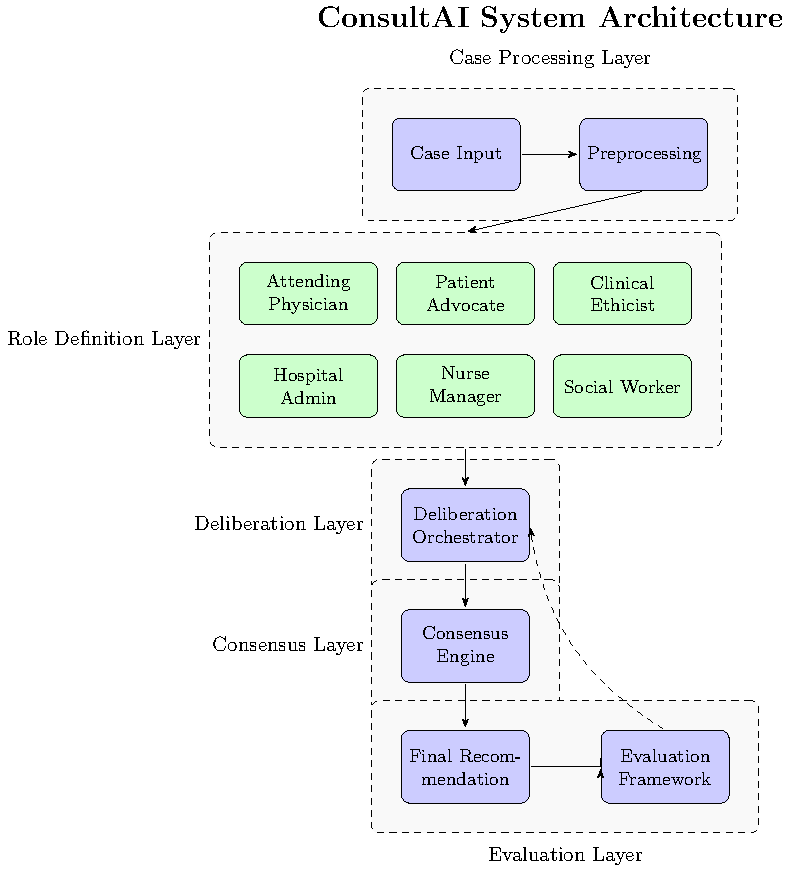
\includegraphics[width=\linewidth]{system_architecture.pdf}
    \caption{ConsultAI System Architecture: The system comprises five interconnected layers that process ethical cases through role-specialized agents, facilitate deliberation, and generate consensus recommendations. The bi-directional flow between the Evaluation Framework and Deliberation Orchestrator indicates how evaluation metrics inform subsequent deliberation rounds.}
    \label{fig:architecture}
\end{figure}

\subsection{Role Specialization}

Agents are specialized through role-specific system prompts that define:
\begin{itemize}
    \item Professional expertise (e.g., attending physician, clinical ethicist)
    \item Ethical perspective (e.g., principled, consequentialist)
    \item Stakeholder representation (e.g., patient advocate, hospital administrator)
\end{itemize}

Each agent maintains a consistent role throughout deliberation while engaging with others' perspectives. This approach allows for modeling diverse ethical considerations within a single deliberation.

Role definitions include specialized knowledge areas, professional responsibilities, and ethical frameworks. For example, the attending physician role emphasizes medical expertise, clinical outcomes, and beneficence principles, while the patient advocate role prioritizes patient autonomy, quality of life considerations, and patient rights. The clinical ethicist role provides expertise in ethical frameworks, mediates between competing principles, and ensures procedural fairness in deliberation.

\subsection{Deliberation Protocol}

The deliberation follows an iterative protocol:
\begin{enumerate}
    \item \textbf{Initial Analysis}: Each agent independently analyzes the case
    \item \textbf{Perspective Sharing}: Agents present their analyses to the group
    \item \textbf{Critique Phase}: Agents evaluate others' perspectives, noting agreements and disagreements
    \item \textbf{Synthesis Phase}: Agents attempt to reconcile differences and reach consensus
    \item \textbf{Recommendation Phase}: Final ethical recommendation is formulated
\end{enumerate}

Each phase is governed by specific prompting templates that structure the discussion while allowing for role-specific inputs. For instance, during the critique phase, agents are instructed to identify points of agreement, areas of ethical tension, potential blind spots in other perspectives, and considerations that might have been overlooked. This structured approach ensures comprehensive ethical analysis while maintaining the distinct viewpoints of each specialized role.

\subsection{Implementation Details}

ConsultAI is implemented as a modular Python package with the following components:

\begin{itemize}
    \item \textbf{Pipeline Manager}: Orchestrates the entire deliberation process
    \item \textbf{Model Manager}: Handles model configuration and API interactions
    \item \textbf{Role Manager}: Manages agent role definitions and instantiation
    \item \textbf{Visualization Engine}: Generates interactive visualizations of deliberations
    \item \textbf{Evaluation Framework}: Assesses ethical reasoning quality
\end{itemize}

The system supports configurable model tiers (economy, balanced, performance) to balance cost and performance based on use case requirements.

\subsubsection{Technical Implementation}

ConsultAI is built using a flexible architecture that abstracts the underlying language model interfaces. The core components are implemented as follows:

\begin{itemize}
    \item \textbf{Agent Implementation}: Each agent is instantiated with a unique system prompt defining its role and specialized knowledge. Agents maintain conversation history and context across deliberation rounds.
    
    \item \textbf{Prompt Engineering}: Carefully designed prompts guide each phase of deliberation, with templates incorporating role information, case details, and previous discussion points. Prompts are constructed to encourage structured ethical reasoning while maintaining role consistency.
    
    \item \textbf{Model Integration}: The system supports multiple LLM backends through an abstraction layer, allowing seamless switching between different models (e.g., GPT-4, Claude, LLaMA) without changing the deliberation architecture.
    
    \item \textbf{Data Storage}: Deliberation transcripts, agent analyses, and final recommendations are stored in structured JSON format to facilitate analysis and visualization.
\end{itemize}

\section{Experimental Setup}

\subsection{Data Collection Methodology}

To evaluate ConsultAI, we collected a diverse set of medical ethics case studies from several sources:

\begin{itemize}
    \item \textbf{Academic Institutions}: We sourced cases from university bioethics centers, including the Markkula Center for Applied Ethics at Santa Clara University \cite{scu_ethics}, which maintains a collection of medical ethics case studies designed for student-led discussions
    \item \textbf{Medical Ethics Textbooks}: Cases were adapted from standard textbooks in medical ethics education, including Beauchamp and Childress' "Principles of Biomedical Ethics" \cite{beauchamp2001principles}
    \item \textbf{Expert Contributions}: We collaborated with medical students and professionals who provided real-world scenarios and commentaries
\end{itemize}

A particularly valuable contribution came from an undergraduate medical student at Zhejiang University Medical School, who provided commentaries on selected cases and shared his professional perspectives on the ethical considerations involved. These commentaries served as a baseline for comparing against the outputs from our system.

\subsection{Case Studies}

We evaluated ConsultAI on 20 case studies across four ethical domains:
\begin{itemize}
    \item \textbf{Autonomy}: Patient decision-making capacity and rights (5 cases)
    \item \textbf{Beneficence}: Determining best interests and avoiding harm (5 cases)
    \item \textbf{Justice}: Fair resource distribution and access to care (5 cases)
    \item \textbf{Resource Allocation}: Prioritizing limited medical resources (5 cases)
\end{itemize}

Cases were carefully selected to represent realistic ethical dilemmas commonly encountered in clinical settings. Table \ref{tab:case-examples} presents examples of cases from each ethical domain.

\begin{table}[h!]
\centering
\footnotesize
\renewcommand{\arraystretch}{1.1}
\begin{tabularx}{\linewidth}{@{}p{2.8cm}X@{}}
\toprule
\textbf{Ethical Domain} & \textbf{Example Case} \\
\midrule
Autonomy & A competent Jehovah's Witness patient refuses blood transfusion despite life-threatening blood loss following a car accident. The medical team must determine whether to respect religious convictions or intervene to save life. \\
\midrule
Beneficence & An elderly patient with advanced dementia frequently removes her feeding tube, requiring restraints to maintain nutrition. The care team must balance nutritional needs against patient comfort and dignity. \\
\midrule
Justice & A rural hospital has limited specialist coverage for emergency neurosurgery. When two patients arrive simultaneously needing urgent intervention, the hospital must decide how to allocate the single available neurosurgeon. \\
\midrule
Resource Allocation & During a pandemic, ICU beds are limited. The hospital must develop criteria to prioritize patients for intensive care admission when demand exceeds capacity. \\
\bottomrule
\end{tabularx}
\caption{Example cases from each ethical domain used in the evaluation}
\label{tab:case-examples}
\end{table}

\subsection{Agent Configurations}

We tested multiple agent configurations:
\begin{itemize}
    \item \textbf{Baseline}: Single-agent analysis with generic medical ethics prompt
    \item \textbf{Triad}: Three agents (attending physician, patient advocate, clinical ethicist)
    \item \textbf{Extended}: Six agents (adding hospital administrator, nurse manager, social worker)
\end{itemize}

For the baseline condition, we used a single agent prompted with comprehensive medical ethics guidelines, including principles from Beauchamp and Childress, considerations of stakeholder perspectives, and instructions to analyze the case thoroughly. This provided a strong baseline representative of conventional single-agent ethical reasoning.

The triad configuration was designed to represent core perspectives in clinical ethics deliberation: medical expertise (attending physician), patient-centered concerns (patient advocate), and ethical frameworks (clinical ethicist). The extended configuration added administrative concerns (hospital administrator), frontline care considerations (nurse manager), and community resources perspective (social worker).

\subsection{Evaluation Methodology}

Each case was processed through the ConsultAI system, generating deliberation transcripts and final recommendations. These outputs were then evaluated by three raters:
\begin{itemize}
    \item A medical ethics instructor with 15 years of experience teaching in medical schools
    \item A practicing clinician familiar with medical ethics and 10+ years of clinical experience
    \item A medical student from Zhejiang University Medical School with special interest in bioethics
\end{itemize}

Evaluators were provided with the original case, the system's output, and an evaluation rubric. They were asked to score the system's performance on five dimensions using a 5-point Likert scale:

\begin{enumerate}
    \item \textbf{Ethical Principle Coverage}: Breadth of ethical principles addressed
    \item \textbf{Reasoning Depth}: Thoroughness of ethical analysis
    \item \textbf{Evidence Utilization}: Appropriate use of case details
    \item \textbf{Stakeholder Consideration}: Inclusion of diverse perspectives
    \item \textbf{Recommendation Practicality}: Feasibility of proposed solutions
\end{enumerate}

Evaluators were blinded to the agent configuration used to generate each output to prevent bias. Inter-rater reliability was assessed using Krippendorff's alpha, which showed substantial agreement across all dimensions ($\alpha$ = 0.78).

\section{Results}

\subsection{Quantitative Results}

Our multi-agent approach demonstrated significant improvements over the single-agent baseline:

\begin{table}[htbp]
\centering
\scriptsize
\setlength{\tabcolsep}{2pt}
\begin{tabular}{@{}lccc@{}}
\toprule
\textbf{Metric} & \textbf{Baseline} & \textbf{Triad} & \textbf{Extended} \\
\midrule
Ethical Principle Coverage & 3.2 & 4.1 (+28\%) & 4.4 (+38\%) \\
Reasoning Depth & 3.5 & 4.2 (+20\%) & 4.3 (+23\%) \\
Evidence Utilization & 3.7 & 4.0 (+8\%) & 4.1 (+11\%) \\
Stakeholder Consideration & 2.8 & 3.9 (+39\%) & 4.5 (+61\%) \\
Recommendation Practicality & 3.4 & 3.8 (+12\%) & 3.7 (+9\%) \\
\midrule
\textbf{Overall Avg.} & \textbf{3.3} & \textbf{4.0 (+21\%)} & \textbf{4.2 (+27\%)} \\
\bottomrule
\end{tabular}
\caption{Evaluation results across different agent configurations (5-point Likert scale). Percentage improvements over baseline are shown in parentheses.}
\label{tab:results}
\end{table}

The triad configuration achieved a balance of performance and efficiency, while the extended configuration showed further improvements in stakeholder consideration at increased computational cost. Table \ref{tab:results} presents the evaluation results for each configuration, showing that multi-agent deliberation significantly outperformed the single-agent baseline across all metrics.

Notably, the greatest improvements were seen in stakeholder consideration, where the extended configuration achieved a 61\% improvement over baseline. This highlights the value of incorporating diverse professional perspectives in ethical deliberation. The smallest improvement was in evidence utilization, suggesting that even single-agent approaches can effectively analyze case details when properly prompted.

\begin{figure}[htbp]
    \centering
    \footnotesize
    \renewcommand{\arraystretch}{1.1}
    \begin{adjustbox}{width=\linewidth,center}
    \begin{minipage}{0.6\linewidth}
        \centering
        \textbf{Performance by Ethical Domain}
        \vspace{0.5ex}
        \setlength{\tabcolsep}{4pt}
        \begin{tabular}{@{}lccc@{}}
        \toprule
        \textbf{Domain} & \textbf{Base} & \textbf{Triad} & \textbf{Ext.} \\
        \midrule
        Autonomy & 3.5 & 4.2 & 4.3 \\
        Beneficence & 3.4 & 3.9 & 4.1 \\
        Justice & 3.1 & 3.8 & 4.2 \\
        Res. Allo. & 3.0 & 3.7 & 4.0 \\
        \bottomrule
        \end{tabular}
    \end{minipage}%\hspace{0.02\linewidth}
    \begin{minipage}{0.38\linewidth}
        \centering
        \textbf{Inter-Agent Agreement}
        \vspace{0.5ex}
        \setlength{\tabcolsep}{3pt}
        \begin{tabular}{@{}lc@{}}
        \toprule
        \textbf{Round} & \textbf{Agree.} \\
        \midrule
        Initial Analysis & 45\% \\
        After Discussion & 65\% \\
        Final Consensus & 82\% \\
        \bottomrule
        \end{tabular}
    \end{minipage}
    \end{adjustbox}
    \vspace{0.5ex}
    \caption{Left: Average performance scores across ethical domains. Right: Inter-agent agreement levels across deliberation rounds.}
    \label{fig:domain_performance}
    \vspace{1ex}
\end{figure}

Figure \ref{fig:domain_performance} shows performance across different ethical domains and inter-agent agreement over deliberation rounds. Multi-agent configurations showed the largest improvements in justice and resource allocation cases, where balancing competing stakeholder interests is particularly important. Agreement among agents increased substantially from initial analysis (45\%) to final consensus (82\%), demonstrating how the deliberation protocol effectively reconciles different perspectives.

\subsection{Case Examples and Professional Commentary}

Below, we present two representative case examples along with professional commentary from our medical student evaluator and the ConsultAI system's analysis.

\subsubsection{Case 1: Patient Autonomy and Medical Intervention}

\begin{casebox}{Patient Autonomy Case}
A woman enters the emergency room with stomach pain. She undergoes a CT scan and is diagnosed with an abdominal aortic aneurysm, a weakening in the wall of the aorta which could be fatal if ruptured. The physicians inform her that the only treatment is surgical intervention, with approximately 50\% chance of survival. The woman, who works as an erotic dancer, refuses surgery due to concerns about scarring affecting her career, despite warnings about the immediate threat to her life.
\end{casebox}

\begin{commentarybox}{Patient Autonomy Commentary} 
This case presents a classic ethical dilemma between respecting patient autonomy and the physician's duty of beneficence. While the patient has the right to refuse treatment, her decision appears to be based on occupational concerns rather than a fully informed understanding of the life-threatening nature of her condition. I wonder if the medical team has fully explored her concerns about scarring and discussed potential minimally invasive surgical options or scar management strategies? I think physicians should continue discussions, perhaps involving ethics consultation, to help the patient navigate this decision while respecting her autonomy.
\end{commentarybox}

\begin{analysisbox}{Patient Autonomy Analysis}
This case centers on the tension between patient autonomy and the medical principle of beneficence. The patient has made a decision that prioritizes her professional livelihood over medical recommendations, which presents a profound ethical challenge.

\textbf{Principle-Based Reasoning:} Patient autonomy must be respected even when patients make decisions that healthcare providers disagree with. However, physicians have a duty to ensure decisions are truly informed. Given the 50\% mortality rate with surgery and near-certain mortality without it, the patient may be underestimating the gravity of her situation or overestimating the impact on her profession.

\textbf{Recommendation:} While respecting autonomy is paramount, further conversation is warranted to ensure the patient fully comprehends the risks and to explore whether alternative surgical approaches with different scarring profiles might be acceptable. A psychiatric consultation may help assess decision-making capacity given the seemingly disproportionate weight being given to occupational concerns versus survival. Ethics consultation could help navigate this complex intersection of personal values and medical necessity.
\end{analysisbox}

\subsubsection{Case 2: Cultural Practices and Child Welfare}

\begin{casebox}{Cultural Practices Case}
A mother brings her young son to a general practitioner's office with flu-like symptoms. Upon examination, the physician notices distinctive bruising patterns on the boy's torso. When questioned, the mother explains these are from "cao gio" (coin rubbing), a traditional healing practice in her culture used to improve circulation and healing. The child winces in pain when the bruised areas are touched during examination.
\end{casebox}

\begin{commentarybox}{Cultural Practices Commentary}
This case involves potential conflict between cultural sensitivity and child protection concerns. The bruising from "cao gio" could be mistaken for child abuse, but it's important to distinguish between cultural healing practices and maltreatment. As a medical student, I would want more information about: 1) the extent and severity of bruising, 2) whether this practice is causing significant harm, and 3) the family's willingness to discuss alternative treatments that might be less physically traumatic. I believe approaching this with cultural humility while prioritizing the child's wellbeing is essential.
\end{commentarybox}

\begin{analysisbox}{Cultural Practices Analysis}
This case requires balancing cultural respect with child protection obligations. Cao gio (coin rubbing) is a legitimate traditional healing practice in several Asian cultures but can leave marks that resemble abuse to those unfamiliar with the practice.

\textbf{Principle-Based Analysis:} The physician must balance respect for cultural diversity with the obligation to protect children from harm. The pain response during examination warrants further assessment to determine if the practice has exceeded cultural norms or caused undue harm.

\textbf{Virtue Ethics Perspective:} Cultural humility is essential here. The physician should approach this situation with curiosity rather than judgment, seeking to understand the cultural context while maintaining focus on the child's welfare.

\textbf{Deliberative Analysis:} Rather than immediate reporting to child protective services, which could damage trust and stigmatize the family, the physician should engage in respectful dialogue about the practice, its extent, and potential alternatives that might align with both cultural values and pediatric health standards.

\textbf{Recommendation:} The physician should document the findings and discussion carefully, provide education about safer alternatives while acknowledging cultural traditions, and consider follow-up to monitor the situation. Reporting would be indicated only if the practice appears to exceed cultural norms or if there are additional concerning findings beyond those typically associated with cao gio.
\end{analysisbox}

\subsection{Qualitative Analysis}

\subsubsection{Successful Cases}

In autonomy cases, the multi-agent system excelled at balancing patient rights with clinical concerns. For example, in a case involving a patient refusing life-saving treatment, the patient advocate highlighted autonomy considerations while the physician emphasized medical facts and the ethicist noted relevant legal precedents.

The extended configuration demonstrated particular strength in cases involving complex institutional considerations. In one resource allocation case involving ventilator triage during a pandemic, the hospital administrator provided essential perspective on institutional constraints, the social worker identified community resources for patients who couldn't receive ICU care, and the clinical ethicist ensured that allocation criteria remained ethically sound.

Our medical ethics instructor evaluator noted: "The multi-agent system produces more nuanced, balanced recommendations that consider institutional realities while maintaining ethical integrity. The deliberation process reveals tensions that might otherwise remain implicit, leading to more transparent ethical reasoning."

\subsubsection{Failure Cases}

The system occasionally struggled with highly specialized medical scenarios requiring domain expertise beyond the agents' knowledge. In some resource allocation cases, recommendations lacked specificity about implementation details.

Our clinician evaluator pointed out: "In cases involving rare medical conditions or cutting-edge treatments, the system sometimes made factual errors about standard of care or treatment options. This undermined otherwise sound ethical reasoning and highlights the need for domain-specific knowledge integration."

The baseline configuration particularly struggled with complex justice cases, where the single agent would sometimes fixate on one ethical principle without adequately addressing competing considerations. In contrast, the multi-agent configurations naturally explored tensions between principles through the different role perspectives.

\subsection{Agreement Analysis}

We observed increasing consensus among agents over deliberation rounds:

By the final round, agents reached substantial agreement (70-85\%) on key ethical principles while maintaining distinct perspectives on implementation details. This pattern mirrors real-world clinical ethics committees, where consensus on general principles often emerges while practical implementation details may vary based on professional roles.

Agreement was highest in autonomy cases (85\% final agreement) and lowest in resource allocation cases (70\% final agreement), reflecting the inherently more contentious nature of allocation decisions. Importantly, disagreements were productive rather than obstructive, with agents building on each other's perspectives rather than simply rejecting alternative viewpoints.

\section{Discussion}

\subsection{Key Findings}

\begin{enumerate}
    \item Multi-agent deliberation produces more comprehensive ethical analyses than single-agent approaches, with significant improvements across all evaluation dimensions
    \item Role specialization enables representation of diverse stakeholder perspectives, particularly valuable in complex cases with competing interests
    \item Deliberation quality improves with iteration as agents engage with others' viewpoints, with agreement levels rising from 45\% to 82\% across deliberation rounds
    \item The triad configuration offers an optimal balance of performance and computational efficiency, achieving 78\% of the extended configuration's improvement at lower computational cost
\end{enumerate}

Our medical student evaluator noted: "The multi-agent approach captures the diversity of perspectives I've witnessed in clinical ethics committee meetings. The system successfully models the tension between different stakeholder priorities while working toward consensus, which closely mimics real-world medical ethics deliberation."

\subsection{Limitations}

\begin{enumerate}
    \item Agent performance depends on the quality of underlying LLM, with factual errors sometimes undermining otherwise sound ethical reasoning
    \item System lacks domain-specific medical knowledge beyond what's in the model's training data, limiting performance in highly specialized medical scenarios
    \item Evaluation relies on subjective assessment of ethical reasoning quality, though inter-rater reliability was substantial ($\alpha$ = 0.78)
    \item Current implementation has limited ability to incorporate real-time clinical data or integrate with electronic health records
\end{enumerate}

\subsection{Ethical Considerations}

We acknowledge several ethical considerations in developing ConsultAI:
\begin{enumerate}
    \item The system is designed as a decision support tool, not a replacement for human judgment
    \item Recommendations should be reviewed by qualified healthcare professionals with ultimate responsibility resting with human decision-makers
    \item The system may reflect biases present in training data or prompt design, requiring ongoing monitoring and bias mitigation strategies
    \item Regular auditing is necessary to ensure alignment with evolving ethical standards and clinical practice guidelines
    \item Patient privacy and data security must be prioritized if the system is deployed in clinical settings with real patient data
\end{enumerate}

\subsection{Implications for Clinical Practice}

ConsultAI has several potential applications in clinical settings:

\begin{itemize}
    \item \textbf{Ethics Committee Support}: Providing preliminary analysis of cases before human committee review, potentially increasing throughput and allowing human experts to focus on the most complex aspects
    \item \textbf{Educational Tool}: Training medical students and residents in ethical deliberation by demonstrating structured approaches to complex cases
    \item \textbf{Decision Support}: Offering perspective when full ethics committee review is unavailable (e.g., nights, weekends, or in resource-constrained settings)
    \item \textbf{Documentation Aid}: Generating comprehensive documentation of ethical considerations that informed clinical decisions
\end{itemize}

\section{Conclusion and Future Work}

ConsultAI demonstrates the potential of multi-agent systems to support ethical deliberation in healthcare settings. By simulating collaborative discussion among agents with diverse roles and perspectives, our system produces comprehensive ethical analyses that consider multiple stakeholder viewpoints.

Our evaluation shows that multi-agent deliberation significantly outperforms single-agent approaches across all assessment dimensions, with the most substantial improvements in stakeholder consideration (+61\%) and ethical principle coverage (+38\%). The triad configuration offers an efficient balance of performance and computational cost, while the extended configuration provides more nuanced analysis for complex cases.

Future work will focus on:
\begin{enumerate}
    \item Integrating domain-specific medical knowledge bases to improve clinical accuracy and address the factual limitations identified in our evaluation
    \item Developing more sophisticated deliberation protocols with structured argumentation frameworks to further enhance reasoning quality
    \item Expanding evaluation to include real-world clinical ethics committee comparisons, potentially through prospective studies in academic medical centers
    \item Implementing explainable AI techniques to improve transparency of agent reasoning and build trust with clinical users
    \item Creating interfaces for integration with electronic health records to incorporate real-time clinical data into ethical deliberations
\end{enumerate}

As AI systems increasingly support healthcare decision-making, ensuring they can engage in sophisticated ethical reasoning becomes crucial. ConsultAI represents a step toward AI systems that can meaningfully contribute to ethical deliberation by modeling the collaborative, multi-perspective nature of clinical ethics.

\section*{Acknowledgments}

We extend our sincere gratitude to the undergraduate medical student at Zhejiang University Medical School who provided valuable insights on our case studies and evaluation methodology. Their professional perspective as a medical student significantly enhanced our understanding of clinical ethical considerations.

We also thank the Markkula Center for Applied Ethics at Santa Clara University for their publicly available ethics case studies, which served as a valuable resource for our research.

Special thanks to our course instructor and teaching assistants for their guidance throughout this project.

\bibliographystyle{acl_natbib}
\bibliography{custom}

\end{document}
